
\todo[inline]{Update introduction  to refer to  Full Run 2 analysis.\\
   			  Push Q/G tagging earlier.\\
			  Mention updated statistical framework.} 


Searches for anomalous dijet events can be sensitive to a large set of models for Beyond the Standard Model (BSM) physics.
This includes new particles arising from additional broken gauge groups,
excitations of Standard Model particles (for instance Kaluza-Klein excitations in models involving extra dimensions),
interactions between dark matter and the Standard Model, and models of quark compositeness.
If any new particles can be produced at hadron colliders then they must couple to Standard Model (SM) partons.
This coupling means the new particles can decay to jets, often dominantly.
The total dijet production rates for such signals can be large even at substantial fractions of the
total hadron collision energy, allowing searches to begin to probe these energy regimes with relatively little data.

For these reasons, searches in dijet events are often amongst of the first searches done when a hadron
collider reaches a new energy frontier\footnote{See Ref.~\cite{Harris:2011bh} for a review of the history
of these searches from UA1 and UA2 to the LHC Run 1.}.  Increases in collision centre-of-mass energy, \s , 
dramatically improves the reach of searches for potential high-mass signals. 
Increases in the integrated luminosity of the data samples results in much smaller improvements and requires significant 
improvements in the understanding of systematic uncertainties. 


A search for new physics both in the dijet mass distribution and in the angular distributions was performed on 13~\TeV\xspace data collected in 2015 and 2016 \cite{EXOT-2016-21} with the  95\% CL lower limits on the masses given in Table~\ref{tab:Limits201516}. 
Most of the strategies and methods of the analysis are mostly unchanged with respect to the previous iterations of the analysis, which can be reviewed in great detail in the internal
notes \cite{Bauce:2226443}.


%The increase in collision center-of-mass energy \s\ from
%8 to 13~\TeV\xspace dramatically enhances parton luminosities at multi-\TeV\xspace energies
%(Fig.~\ref{fig:partonluminosity}) and thus the production rates of potential high-mass signals.



\todo[inline]{Table 1. Check latest limits. Mainly interested in Excited Quark limits here.}

\begin{table}[!h]
	\centering
	\caption{The 95\% CL lower limits on the masses of ADD quantum black holes (\textsc{\BlackMax} event generator), \Wprime\ and \Wstar\ bosons, excited quarks, and $Z^\prime$ bosons for selected coupling values from the resonance search, as well as on the scale of contact interactions for constructive ($\eta_{\text{LL}}=-1$) and destructive ($\eta_{\text{LL}}=+1$) interference from the angular analysis. Where an additional range is listed, masses within the range are also excluded.}
	\begin{tabular}{ l c c}
		\toprule
		\multicolumn{1}{c}{Model} & \multicolumn{2}{c}{95\% CL exclusion limit} \\
		\cmidrule(r){2-3}
		&  Observed & Expected \\
		\midrule
		Quantum black hole &  8.9~TeV\xspace  & 8.9~TeV\xspace \\
		\midrule
		\Wprime  & 3.6~TeV\xspace &   3.7~TeV\xspace \\
		\midrule
		\multirow{2}{*}{\Wstar}  & 3.4~TeV\xspace  &    \multirow{2}{*}{~3.6~TeV\xspace}  \\
		&3.77~TeV -- 3.85~TeV & \\		
		\midrule
		Excited quark & 6.0~TeV\xspace  &   5.8~TeV\xspace  \\
		\midrule
		\Zprime ($g_q= 0.1$)  & 2.1~TeV\xspace & 2.1~TeV\xspace \\
		\midrule
		\Zprime ($g_q= 0.2$)  & 2.9~TeV\xspace & 3.3~TeV\xspace \\
		\midrule                                               
		Contact interaction ($\eta_{\text{LL}}= -1$) & 21.8~TeV\xspace\phantom{.} & 28.3~TeV\xspace\phantom{.} \\
		\midrule
		\multirow{2}{*}{Contact interaction ($\eta_{\text{LL}}= +1$)}  & 13.1~TeV\xspace\phantom{.} & \multirow{2}{*}{15.0~TeV\xspace\phantom{.}} \\
		& 17.4~TeV\xspace\ -- 29.5~TeV\xspace & \\
		\bottomrule
	\end{tabular}
	\label{tab:Limits201516}
\end{table}


If the resonant data sample can be separated  based on the type of  parton that initiated the jets the 
sensitivity of the search should be significantly increased. The fraction of events as a function of 
the dijet mass from QCD  simulated with a  \textsc{Pythia~8.186}~\cite{pythia8} and the leading-order NNPDF2.3~\cite{Ball:2012cx} parton distribution functions (PDFs) is shown in Fig.~\ref{fig:quarkgluonfraction}. 
This suggests that tagging quark and gluon jets should be able to improve the sensitivity of searches for new particles. 
ATLAS has 
published a study \cite{ATL-PHYS-PUB-2017-009} showing that jets can be tagged as quark or gluon jets 
based on the number of charged particles with transverse momentum (\pt ) above 500\,MeV. 
In this note we present the analysis for the whole combined 2015 and 2016 13~\TeV\xspace dataset using quark 
and gluon tagging  based on charged-particle constituent multiplicity.


\todo[inline]{Update Fig 1 with dijet fractions nicer plot...}
\begin{figure}[htb]
 \centering
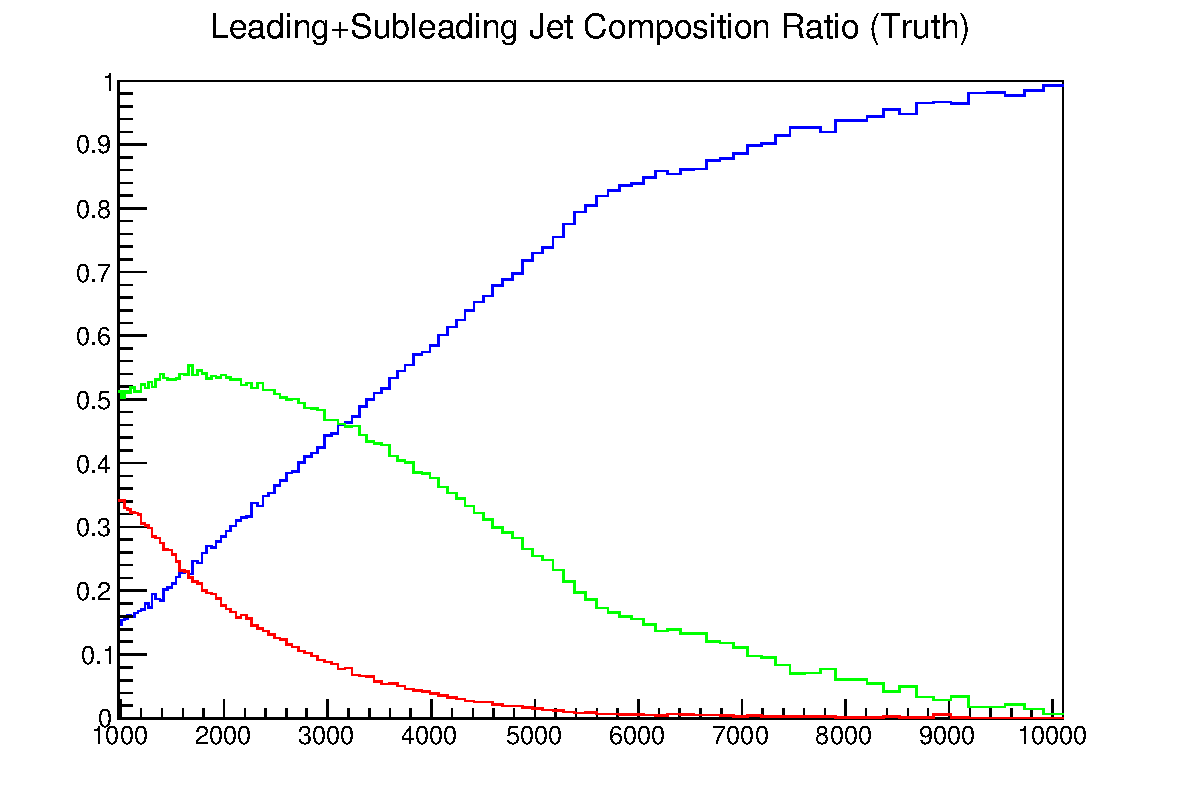
\includegraphics[width=0.75\textwidth]{figures/introduction/truthCompositionRatio.pdf}
\caption{The fraction of dijet events that are initiated by quark-quark events (blue), quark-gluon 
events (green) and gluon-gluon events (red) in simulated data.  \label{fig:quarkgluonfraction}}
\end{figure}

\subsection{Overview of the analysis}
\label{sec:overview}

First, we demonstrate using toy MCs that tagging quark and gluon jets can, in principle, make significant 
improvements to the sensitivity of the resonance search.

The subsequent analysis of the data will follow previously used in the analysis of the 2015 and 2016 data 
\cite{EXOT-2016-21,Bauce:2226443}. This is reproduced here for convinience. 


We analyze dijet events using the dijet invariant mass \mjj\  (described in Section \ref{sec:observables}).

The initial analysis steps are

\begin{enumerate}
\item Unprescaled single-jet triggers are used to collect events containing
highly energetic jets (Section~\ref{sec:trigger})
\item High-\pT\xspace jets are reconstructed, identified, and calibrated according to recommendations, with techniques
prepared in tandem between the analysis team and the
JetEtMiss group (Section~\ref{sec:jet_reconstruction}).
\item After calibration, bulk processing of the data, and production of a standardized xAOD derivation, events are selected with very similar kinematic 
criteria as in previous dijet searches (Section~\ref{sec:event_selection}). The data and Monte Carlo used are described in
Section~\ref{sec:benchmark_signals}. Prior to the availability of the data in the final
analysis, analyzers closely monitor the on-line and offline data preparation and
quality efforts for advance warning of problems.%(Appendix~\ref{app:dqchecks}).
\item When the data are available for inclusion in the analysis, the jet kinematics, calibration performance, 
and quality are monitored at the analysis level with a set of studies (Sections~\ref{sec:jet_reconstruction}).
\end{enumerate}


Statistical tests are employed in a
\textit{search phase}, described in Section~\ref{sec:background_estimation_search}, to determine whether the 
data are compatible with a background expectation. 
A localized excess (i.e. a bump) on the smooth \mjj\  distribution
is the target of the resonance analysis.
The background model is derived from a fit to the \mjj\ distribution.
A single localized excess will not bias
this fit in a significant way. The
search phase in the angular method is designed for non-resonant
signals, deriving the background model from Monte Carlo (MC)
simulation. 
The background estimation strategy is described in Section~\ref{sec:background_estimation}.
A description of systematic uncertainties can be found in 
Sections~\ref{sec:systematics_backgrounds} and \ref{sec:systematics_signal}. 
In case either method observes a significant excess, additional tests in the search phase
are detailed in Section~\ref{sec:cross_checks}. The results of the
search phase are shown in Section~\ref{sec:search_results}.

If no new phenomena is found, a ~\textit{limit setting phase} is used
to constrain a set of signals: 
\begin{itemize}
 \item Limits on benchmark signals:
\begin{itemize}
 \item Excited quarks - a benchmark resonant signal.
 \item Contact interactions- the standard benchmark of new, non-resonant phenomena.
 \item Limits on Quantum Black Holes (QBH).
 \item Limits on hadronically decaying \Wprime .
 \item Limits on hadronically decaying \Wstar .
 \item Limits on dark-matter inspired \Zprime\ models.
\end{itemize}
 \item Limits on Gaussian-shaped signal templates.
\end{itemize}
The techniques and tools used for the limit setting are described in
Sections~\ref{subsec:limits_mass} for the resonance analysis. The
systematic uncertainties considered on the benchmark signals are
detailed in Section~\ref{sec:systematics_signal}.
Each of the following sections clarifies what is consistent
with the previous iteration and what has been further developed.


 \subsection{Strategy for applying quark-gluon selection to the 2015 and 2016 data.}
 \label{sec:201516data}

The analysis strategy, cuts, and other details were developed and implemented in previous analyses \cite{EXOT-2016-21,Bauce:2226443}.  
The search and limit setting using quark-gluon tagging will take place after the selection criteria 
have been optimised and the expected sensitivity calculated.

When all the quality checks on the subsamples (see Section~\ref{sec:jet_reconstruction})
show physical behaviour, are smooth, and in general agreement
with the simulation we will proceed with the search.
Where appropriate we take the
JES uncertainty into account in our assessment of the agreement
between data and simulation. 
Pythia is only a LO generator
and we are probing a region where the PDF fits do not
have a lot of information so some difference in the shapes
can exist. Therefore we do not put a strict statistical measure
on the compatibility of the kinematic distributions but rather
look for any local features indicative of operational or
calibration issues or non-physical behaviour.


 
\subsection{Strategy for inclusion of new data}
\label{sec:blinding}

Essentially the same methodology will be  applied to the 2017 and 2018 data as is applied to 
the 2015 and 2016 data  (Section \ref{sec:201516data}). When all the quality checks on the 
subsamples (see Section~\ref{sec:jet_reconstruction}) show physical behaviour, are smooth, and 
in general agreement
with the simulation we will proceed with the search.
 
